\chapter{Energy Based Models}
% Authors: Diksha Meghwal, Chiao-Hsun Wang, Imran
% Lecture date: 04/01/2019

\section{Recap}
% Authors: Diksha Meghwal
% Lecture date: 04/01/2019

A quick recap, energy based models(EBMs) are functions that take an input and product a scalar output as a result of some optimization.
In case of unconditional models, you simply need to detect given a $Y$ whether it is trained or not. Eg: image restoration.
In case of conditional models, the model accepts a conditional input $X$ along with $Y$ where $Y$ is the variable you model. Eg: image classification given an image and a label.\\

The energy based models are trained in such a way that they provide low energy for samples in the training data and produce high energy for samples outside the data.
\begin{figure}[!h]
    \centering
    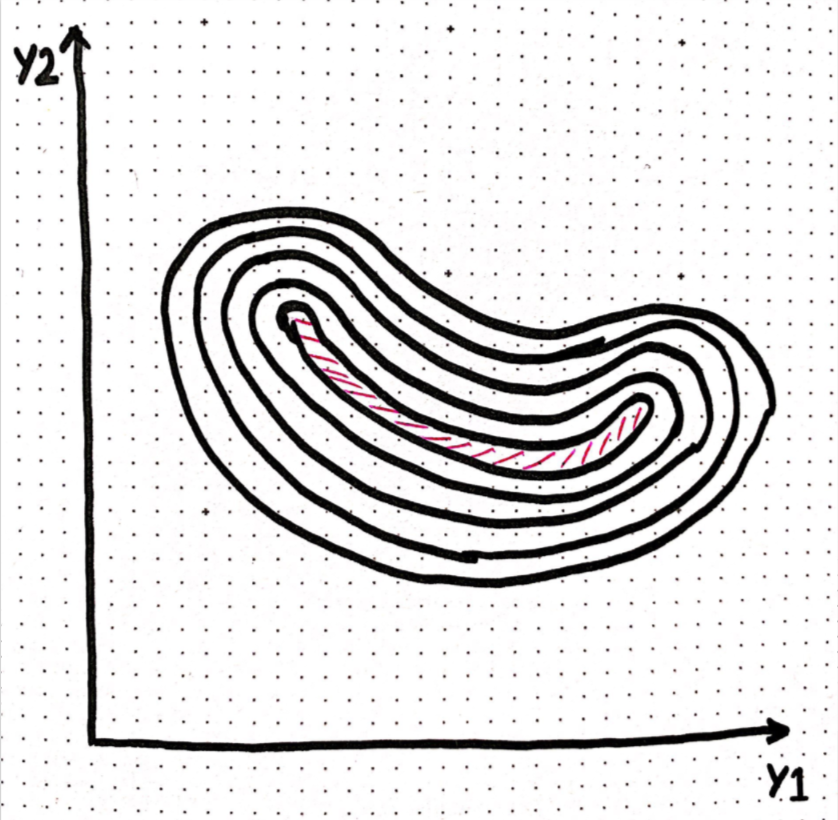
\includegraphics[width=0.4\linewidth]{lectures/08-a/images/EBM_function.png}
    \caption{EBM function}
    \label{fig:EBM_function}
\end{figure}
\section{Latent Variable}
Often energy based models involve a third variable apart from the observed inputs which is not given but modelled into the architecture. These are called latent variables.
\begin{equation}
    F_{w}(Y) = min_{w} E(Y, Z)
\end{equation}
where $Z$ is not given.
\begin{figure}[!h]
    \centering
    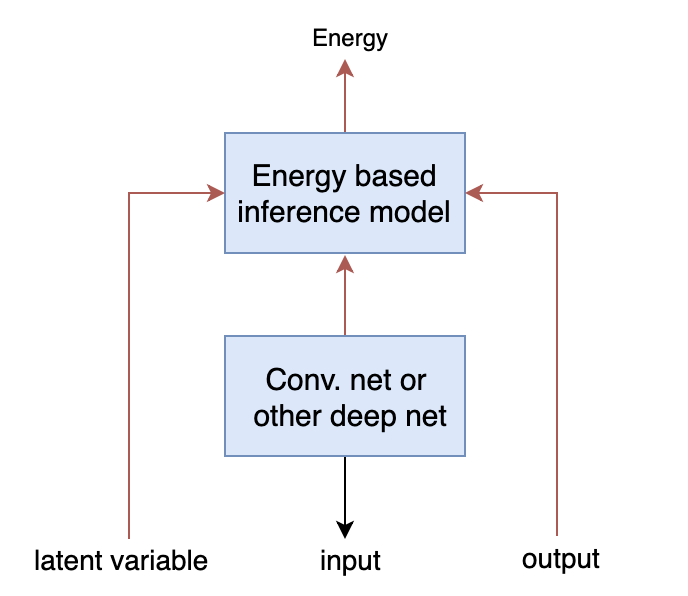
\includegraphics[width=0.4\linewidth]{lectures/08-a/images/latent_EBM_architecture.png}
    \caption{latent EBM model}
    \label{fig:latent_EBM_model}
\end{figure}
\subsection{Examples}
\subsubsection{K-means clustering}
K-means clustering aims to partition n observations into k clusters in which each observation belongs to the cluster with the nearest mean, serving as a prototype of the cluster. This can be modelled as an energy based model where the energy function is given by:
\begin{equation}
    E_{w}(Y,Z) = \left\|Y - WZ \right \|^{2}
\end{equation}
where W is a matrix whose each column represents a prototype and Z is a one hot vector. So the value of this energy function gives the distance between the observed output and the prototype selected by the non-zero element in the vector $Z$.
And the inference for a sample is drawn using the function:
\begin{equation}
    F_{w}(Y) = \min_{Z \in one-hot-vector} E(Y, Z)
\end{equation}
Let 
\begin{equation}
    Z^{*} = \argmin_{Z} E_{w}(Y, Z)
\end{equation}
To calculate the loss function for all the samples we get the loss function:
\begin{equation}
    L(W) = \sum_{i}(F_{w}(Y^{i}))
\end{equation}
Derivating the loss function with respect to W we get:
\begin{equation}
    \frac{d}{dW} L(W) = \sum_{i}-(Y - WZ^{*}) Z^{*T}
\end{equation}
We use the above gradient to update the prototype matrix for each datapoint by considering the prototype that is closest to the datapoint and moving it a little closer to datapoint. Applying batch gradient descent on the above gradient to find the optimal solution gives us the K-means problem.

\subsubsection{Speech Recognition}
Speech recognition is also a classic exmaple of energy based models where the input is a sequence of data and the output is a sequence of feature vectors. We draw inference from these sequence of feature vectors using a language model. The top layer in this case is energy based models like Hidden Markov Chain or recurrent neural networks with some sampling mechanism.

\subsubsection{Keyword Recognition}
Keyword recognition involves detecting limited set of keywords from speech at a very fast rate. We model the problem that given a sequence of voice data, we try to determine the most likely word from the given small corpus. 
\begin{figure}[!h]
    \centering
    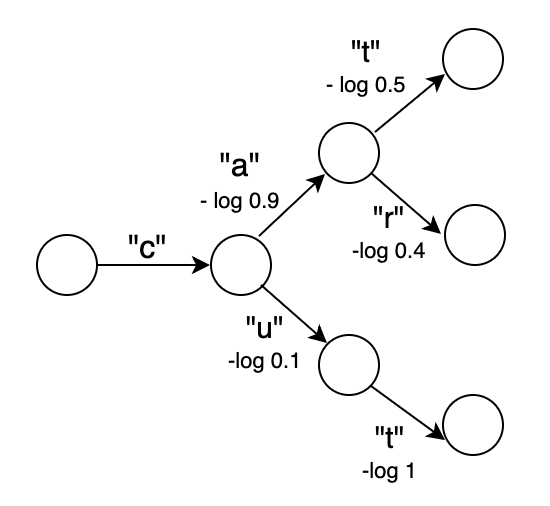
\includegraphics[width=0.4\linewidth]{lectures/08-a/images/keyword model.png}
    \caption{keyword model with the cost for each choice marked on the edge}
    \label{fig:keyword_model}
\end{figure}
We use a small keyword dataset and assign cost to each next possible character in the dataset using a pre-trained language model as shown in the fig \ref{fig:keyword_model}. The cost of the word path is given by the combination of the cost of each step. We use a convolutional neural network or deep net to product cost for every possible sound at every time step and the model combine these energies with the energies provided by the pre-trained model and output the path with minimum cost. In this whole process of finding the solution, the latent variable is the cost of the path.

\subsubsection{Semantic Segmentation}
Semantic segmentation problems require that certain properties are maintained between the input and the output. We can force these restrictions using energy based models which give high energy to small areas of pixels that have a different category as compared to pixels of the large surrounding area. This ensures that there is some uniformity of categories in the output and the input.

\subsection{Marginalization}
As discussed earlier, for certain problems for whom the cumulative probability distribution converges,  we can use a probabilistic model based on Boltzmann distribution to draw the inference.
Considering the probability function:
\begin{equation}
    P(Y|X) = \dfrac{\exp^{-\beta F(X, Y)}}{\int_{y}\exp^{-\beta F(x,y)}}
\end{equation}
This equation can be re-written as:
\begin{equation}
    \int_{z}P(Y,Z|X) = \dfrac{\int_{z} \exp^{-\beta E(X,Y,Z)}}{\int_{y}\int_{z}\exp^{-\beta E(x,y,z)}}
\end{equation}
where Z is the latent variable. We now write this as:
\begin{equation}
    \int_{z}P(Y,Z|X) = \dfrac{\int_{z} \exp^{-\beta F(X,Y)}}{\int_{y}\exp^{-\beta F(x,y)}}
\end{equation}
where F is given by:
\begin{equation}
    F(X,Y) = -\dfrac{1}{\beta} \log \int_{z}\exp^{-\beta E(x,y,z)}
\end{equation}
Thus inference can be obtained by energy minimization over Y and Z given X.
The thing to note here is that the value of value of F(X,Y) is parameterised by $\beta$ and when $\lim_{\beta \to\infty} F_{\beta}(X,Y)$, the only terms that matter are those Y,Z in the power of $\exp$ which give the minimum value for energy,i.e.,:
\begin{equation}
    \lim_{\beta \to\infty} F_{\beta}(X,Y) = \min_{Z} E(X,Y,Z)
\end{equation}
As a result, in marginalization we end up combining all the values for all values of Z for a given Y that give the minimum energy as opposed to a simple probability based inference model where we just pick one value for a given X,Y.

\section{Training an Energy Based Model}
% Authors: Chiao-Hsun Wang
% Lecture date: 4/01/2019

Energy based models can be summarize with the following procedure
\begin{enumerate}
    \item Design an architecture: Decide the form of E(W, Y, X)
    \item Pick an inference algorithm: Decide the method to find Y that minimize E(W, Y, X)
    \item Pick a loss function: Decide the function that measures E(W, Y, X)
    \item Pick an optimization method: Decide The method for finding W that minimizes $\mathcal{L}$
\end{enumerate} 

An important problem is how to decide the loss function for energy based models.
Our goal is to design a loss function $\mathcal{L}$ in such a way that
when we minimize the loss functions with respect to the parameters W,
the effect is that the energy function will give low energy to correct outputs 
and high energy to incorrect outputs.\\

\begin{figure}[h]
    \centering
    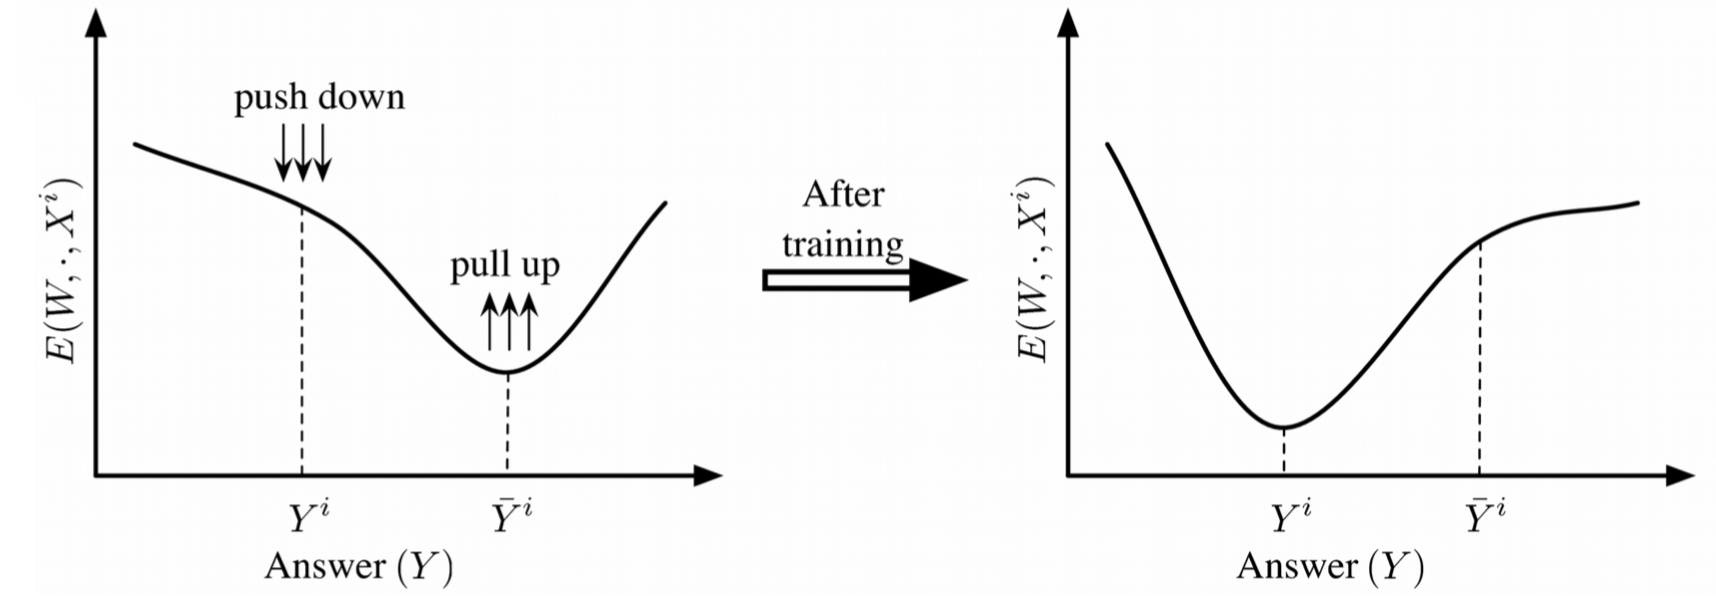
\includegraphics[width=300pt]{lectures/08-a/images/ebm_train.png}
    \caption{The effect of training on energy based models}
    \label{fig:energy_based_models_training}
\end{figure}

Formally, in a training process we have
\begin{itemize}
    \item Family of energy functions: $\mathcal{E} = {E(W,Y,X):X \in \mathcal{W}}$
    \item Training set: $\mathcal{S} = \{(X^i, Y^i): i = 1,...,P \}$
    \item Loss functional: $\mathcal{L}(E, \mathcal{S})$
    \item Training procedure: $W^* = \min_{W \in \mathcal{W}} \mathcal{L}(W, \mathcal{S})$
\end{itemize}

The loss functional has the following form,
\[
    \mathcal{L}(E, \mathcal{S}) = \frac{1}{P} \sum_i^P L(Y^i, E(W, \mathcal{Y},X^i)) + R(W)    
\]
where R is the regularizer. We will introduce different kind of loss functions
in the following sections\\


\subsection{Energy Loss}

A simple example for loss function is the energy loss. For a given training sample
$(X^i,Y^i)$, the loss is defined as
\[
    \mathcal{L}_{energy}(Y^i, E(W, \mathcal{Y}, X^i)) = E(W, Y^i, X^i)    
\]
Minimize the loss function corresponds to pulling down the energy of 
the correct answer. The problem is that training with the loss function won't
necessarily pull up the energy with respect to incorrect answers, which 
leads to a collapsed solution in some cases, 
where the model learns to set the energy as zero. 

\subsection{Negative Log-likelihood Loss}

The negative log-likelihood loss is defined as
\[
    \mathcal{L}_{nll}(W \mathcal{s}) = \frac{1}{P} \sum_i^P (E(W, Y^i, X^i) 
    + \frac{1}{\beta} \log \int_{y \in \mathcal{Y}} e^{-\beta E(W, y, X^i)}
\]

The idea is to maximize the conditional probabilities of all the
correct outputs Y given the input X in the training set, 
\[
    P(Y^1, Y^2, ..., Y^p |X^1, ..., X^p, W)
\]
Assuming the samples are independent and use Gibbs distribution
to transform energy into probabilities,
\[
    P(Y|X^i, W) = \frac{e^{-\beta E(W, Y, X^i)}}
    {\int_{y \in \mathcal{Y}}e^{-\beta E(W, y, X^i)}}    
\]
we will result in the equation
for negative log-likelihood loss.\\

The gradient of the negative log-likelihood loss for a single sample is 
\[
    \frac{\partial{\mathcal{L}(W, Y^i, X^i)}}{\partial{W}}
    = \frac{\partial{E(W, Y^i, X^i)}}{\partial{W}}
    - \int_{Y \in \mathcal{Y}} \frac{\partial{E(W, Y^i, X^i)}}{\partial{W}} P(Y|X^i, W)
\]
where $P(Y|X^i, W)$ is the Gibbs distribution.\\

\subsection{Perceptron Loss}

The perceptron loss is defined as 
\[
    \mathcal{\mathcal{L}}_{\text{perceptron}}(Y^i, E(W,\mathcal{Y}, X^i))
    = E(W, Y^i, X^i) - \min_{y \in \mathcal{Y}} E(W, Y, X^i)
\]

The intuition is from the perceptron algorithm,
which can be viewed as an energy based model.
\begin{itemize}
    \item Energy: $E(W, Y, X) = -YG_W(X)$
    \item Inference: $Y^* = sign(G_W(X))$
    \item Loss: $\mathcal{\mathcal{L}}_{\text{perceptron}}(W, \mathcal{S})
     = \frac{1}{P} \sum_{i=1}^P(sign(G_W(X^i))-Y^i)G_W(X^i)$
    \item Learning Rule: $W \leftarrow W + \eta (Y^i -sign(G_W(X^i)))
    \frac{\partial{G_W(X^i)}}{\partial{W}}$
\end{itemize}

The problem for perceptron loss is similar to energy loss,
where it may produce flat energy surface for certain cases.

\subsection{Generalized Margin Loss}

There are several loss functions that are described as general margin loss.
To introduce the concept, we need to first gives the definition 
to the "Most offending Incorrect Answer"\\

\textbf{Definition: } Let Y be a discrete variable. Then for a training sample $(X^i, Y^i)$,
the most offending incorrect answer $\bar{Y}^i$
is the answer that has the lowest energy among all answers that are incorrect:
\[
    \bar{Y}^i = \text{argmin}_{y \in \mathcal{Y}, Y \neq Y^i}
    E(W, Y, X^i)
\]
\\
\textbf{Definition: } Let Y be a continuous variable. 
Then for a training sample $(X^i, Y^i)$,
the most offending incorrect answer $\bar{Y}^i$
is the answer that has the lowest energy among all answers
that are at least $\epsilon$ away from the correct answer:
\[
    \bar{Y}^i = \text{argmin}_{y \in \mathcal{Y}, \parallel	Y-Y^i\parallel > \epsilon}
    E(W, Y, X^i)
\]
\\
Now we give several examples for generalized marginal loss.
\begin{itemize}
    \item Hinge Loss: 
    $L_{hinge}(W, Y^i, X^i) = \max(0, m + E(W, Y^i, X^i) - E(W, \bar{Y}^i, X^i))$
    \item Log Loss:
    $L_{log}(W, Y^i, X^i) = \log(1 + e^{E(W, Y^i, X^i) - E(W, \bar{Y}^i, X^i)})$
    \item Square-Square Loss:
    $L_{sq-sq}(W, Y^i, X^i) = E(W, Y^i, X^i)^2 + (\max(0, m - E(W, \bar{Y}^i, X^i)))^2$

\end{itemize}

Here is a table that summarize some of the loss functions for energy based models.
\begin{figure}[h]
    \centering
    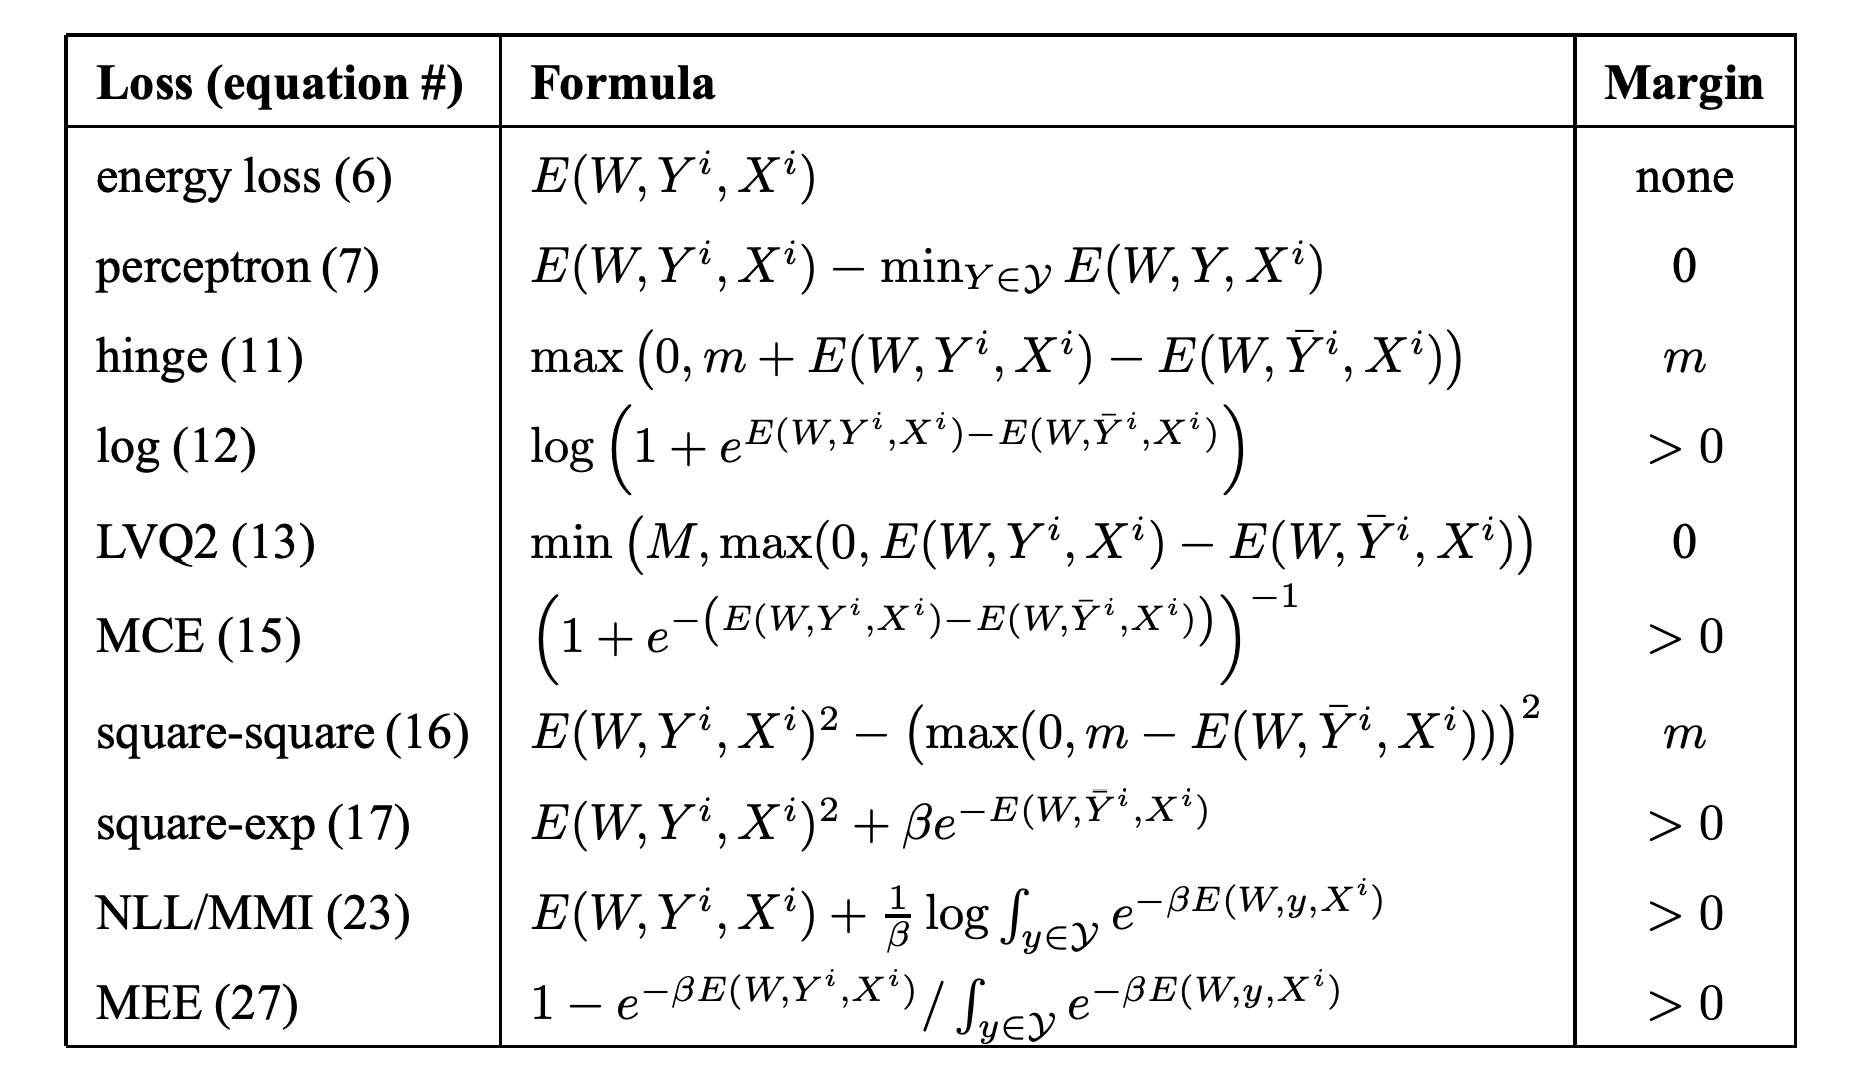
\includegraphics[width=300pt]{lectures/08-a/images/loss_zoo.png}
    \caption{Different loss functions}
    \label{fig:energy_based_models_loss_functions}
\end{figure}


